\textbf{See the instruction for questions \inteval{\value{question}+1} to \inteval{\value{question}+2}.}

\begin{figure}[H]
    \center
    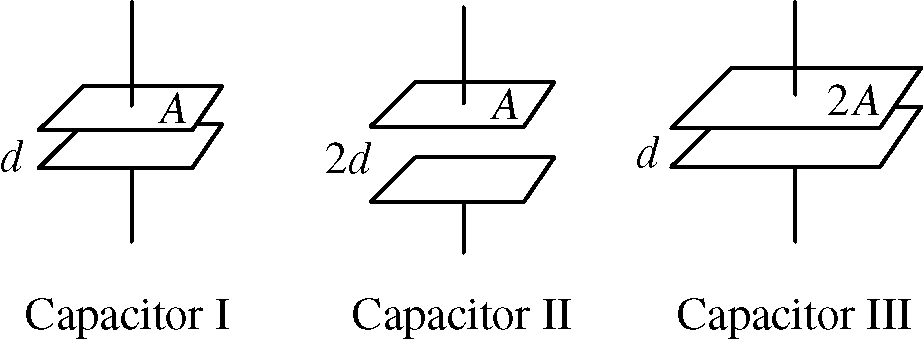
\includegraphics[scale=0.25]{images/img-005-012.png}
\end{figure}

The plate areas and separations for three capacitors are shown in the diagram above. The space between the plates in each capacitor is filled with air.

% Multiple Choice Question 10
\begin{questions}\setcounter{question}{9}\question
Suppose all three capacitors have charge $+Q$ on the top plate and charge $-Q$ on the bottom plate. Which of the following is true of the potential difference across the plates of the three capacitors?

\begin{choices}
\choice It is greatest for I.
\choice It is greatest for II.
\choice It is greatest for III.
\choice It is the same for II and III and least for I.
\choice It is the same for all three capacitors.
\end{choices}\end{questions}

% Multiple Choice Question 11
\begin{questions}\setcounter{question}{10}\question
Suppose all three capacitors are connected in parallel with a $9\unit{V}$ battery. Which of the following is true of the electric field between the plates?

\begin{choices}
\choice It is greatest for I.
\choice It is greatest for II.
\choice It is greatest for III.
\choice It is the same for I and III and least for II.
\choice It is the same for I and II and least for III.
\end{choices}\end{questions}

